% ===================================================================
% 文件名: tex/demo/main.tex
% 用途: TinyTeX 全栈环境自检报告 (含学术增强功能)
% ===================================================================
\PassOptionsToPackage{fontset=fandol}{ctex}
\documentclass[a4paper, 12pt]{article}

% --- 基础环境 ---
\usepackage{ctex}
\usepackage{iftex}
\usepackage{amsmath, amsfonts, amssymb}
\usepackage{newtxtext, newtxmath}
\usepackage[margin=2.5cm]{geometry}
\usepackage{xcolor}
\usepackage{graphicx}
\usepackage{mwe}

% --- [Group 6 新增功能测试包] ---
\usepackage{fancyhdr}       % 页眉页脚
\usepackage{setspace}       % 行距
\usepackage{algorithm}      % 算法浮动体
\usepackage{algpseudocode}  % 伪代码
\usepackage{longtable}      % 跨页表格
\usepackage{threeparttable} % 表格注脚
\usepackage{mhchem}         % 化学公式
\usepackage{pdfpages}       % 插入PDF (仅测试加载)

% --- 其他功能 ---
\usepackage{booktabs, multirow, makecell}
\usepackage{caption, subcaption}
\usepackage{listings, siunitx}
\usepackage{tikz}
\usepackage[colorlinks=true, linkcolor=blue]{hyperref}

% --- 页眉页脚设置 ---
\pagestyle{fancy}
\fancyhead[L]{TinyTeX 自检}
\fancyhead[R]{学术增强版}

% --- 伪代码设置 ---
\floatname{algorithm}{算法}
\renewcommand{\algorithmicrequire}{\textbf{输入:}}
\renewcommand{\algorithmicensure}{\textbf{输出:}}

\title{\textbf{TinyTeX 学术全能版测试}}
\author{CI/CD Bot}
\date{\zhtoday}

\begin{document}

\maketitle

% 设置 1.5 倍行距
\onehalfspacing

\section{学术论文增强功能测试 (Group 6)}

\subsection{伪代码排版 (Algorithmicx)}
测试计算机类论文必备的算法环境:
\begin{algorithm}[H]
    \caption{欧几里得算法 (Euclid's Algorithm)}
    \begin{algorithmic}[1]
        \Require 两个整数 $a, b$
        \Ensure 最大公约数 $\gcd(a, b)$
        \State $r \gets a \bmod b$
        \While{$r \ne 0$}
            \State $a \gets b$
            \State $b \gets r$
            \State $r \gets a \bmod b$
        \EndWhile
        \State \Return $b$
    \end{algorithmic}
\end{algorithm}

\subsection{化学公式 (mhchem)}
测试理工科常用的化学式排版:
\begin{itemize}
    \item 水的电离:\ce{2H2O <=> H3O+ + OH-}
    \item 沉淀反应:\ce{SO4^2- + Ba^2+ -> BaSO4 v}
\end{itemize}

\subsection{复杂表格增强}

\subsubsection{带注脚的表格 (ThreePartTable)}
\begin{table}[htbp]
    \centering
    \begin{threeparttable}
        \caption{实验数据统计}
        \begin{tabular}{lcc}
            \toprule
            组别 & 均值 & 标准差 \\
            \midrule
            对照组 & 12.5 & 0.8 \\
            实验组 & 14.2\tnote{*} & 1.1 \\
            \bottomrule
        \end{tabular}
        \begin{tablenotes}
            \footnotesize
            \item[*] 表示 $P < 0.05$ (显著差异).
        \end{tablenotes}
    \end{threeparttable}
\end{table}

\subsubsection{跨页长表格 (Longtable)}
(这里模拟一个可能会跨页的表格环境,验证宏包加载)
\begin{longtable}{p{3cm} p{8cm}}
    \caption{长表格测试}\\
    \toprule
    \textbf{字段} & \textbf{说明} \\
    \midrule
    \endfirsthead
    \multicolumn{2}{c}{续表...}\\
    \midrule
    \endhead
    \bottomrule
    \endlastfoot
    
    FancyHDR & 用于定制页眉页脚,学位论文必备。 \\
    SetSpace & 用于调整行距,如学位论文要求的 20 磅行距。 \\
    PdfPages & 用于插入签署好的独创性声明扫描件。 \\
    LongTable & 用于附录中展示冗长的实验数据或符号表。 \\
\end{longtable}

\section{基础功能回归测试}
\begin{itemize}
    \item \textbf{中文字体}:Fandol 宋体/黑体显示正常。
    \item \textbf{数学字体}:$\oint \mathbf{E} \cdot d\mathbf{l}$ (Times 风格)。
    \item \textbf{TikZ 绘图}:
    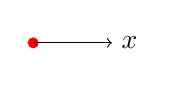
\begin{tikzpicture}[baseline=-3pt]
        \fill[red] (0,0) circle (2pt);
        \draw[->] (0,0) -- (1,0) node[right] {$x$};
    \end{tikzpicture} 绘图引擎正常。
\end{itemize}

\end{document}